\documentclass[journal]{IEEEtran}

% --- DODANE PACZKI ---
\usepackage{graphicx}
\usepackage{booktabs} % Dla \toprule, \midrule, \bottomrule w tabelach
\usepackage{amsmath}
\usepackage{cite}
\usepackage{url}
\usepackage[hidelinks]{hyperref}
\usepackage{multirow}
\graphicspath{{Fig/}}

% Prawidłowe łamanie wyrazów
%\hyphenation{op-tical net-works semi-conduc-tor}

\begin{document}

\title{Relative Logistic Regression: A Probabilistic Refinement of Hard-Voting Pair-Based Omics Classification}

\author{Marcin~Czajkowski,
        Anna~Czajkowska,
        Krzysztof~Jurczuk,
        and~Marek~Kretowski%
\thanks{M. Czajkowski, K. Jurczuk, and M. Kretowski are with the Faculty of Computer Science, Bialystok University of Technology, 15-351 Bialystok, Poland (e-mail: m.czajkowski@pb.edu.pl).}%
\thanks{A. Czajkowska is with the Department of Medical Biology, Medical University of Bialystok, Bialystok, Poland.}}

\maketitle

\begin{abstract}
Pair-based classifiers such as Top-Scoring Pairs (TSP) and k-Top-Scoring Pairs (k-TSP) are attractive for omics classification because they use interpretable within-sample feature orderings and are less dependent on absolute measurement scales. However, their classical aggregation rule assigns equal weight to all retained pairs and produces coarse vote-derived scores with limited probabilistic resolution.

We introduce Relative Logistic Regression (RLR), an integrated pair-based pipeline combining supervised pair ranking, gene-disjoint shortlist construction, ternary rank-margin encoding of within-sample gene-pair relations, and sparse elastic-net logistic fitting. The resulting model can assign unequal fitted contributions to shortlisted relations, shrink uninformative relations to zero, and distinguish the nominal shortlist from the globally fitted and locally active relational structure.

RLR was evaluated in four complementary settings: a repeated benchmark across 11 transcriptomic datasets for primary comparative inference, a fixed-split pulmonary tuberculosis (PTB) public-cohort case study for structural inspection, a leave-one-cohort-out PTB stress test, and a classical eight-dataset microarray benchmark for historical positioning. Relative to the corresponding classical k-TSP configurations at the same nominal pair-signature sizes, the most consistent improvements were observed in logloss, with supporting reductions in Brier score and expected calibration error. Differences in AUC and F1 were smaller and mixed, indicating that the main benefit concerns probability quality rather than universal improvement in discrimination. Post-hoc calibration reduced part of the gap between vote-derived k-TSP scores and RLR, but did not remove it in the intermediate and larger configurations.

In the PTB case study, RLR preserved an inspectable pair-based signature while assigning unequal weights and shrinking selected relations from the fitted decision structure. Overall, RLR is best interpreted as a probabilistic refinement of pair-based omics classification that improves score resolution while retaining an explicitly relational and structurally inspectable representation.
\end{abstract}

\begin{IEEEkeywords}
omics classification; pair-based classification; relative expression analysis; top-scoring pairs; probabilistic modeling; interpretable machine learning
\end{IEEEkeywords}

\IEEEpeerreviewmaketitle
%%%%%%%%%%%%%%%%%%%%%%%%%%%%%%%%%%%%%%%%%%

\section{Introduction}

\IEEEPARstart{H}{igh-dimensional} omics classification remains challenging because the number of measured features typically far exceeds the number of available samples, while cohort heterogeneity, platform effects, and study-specific preprocessing can complicate model transfer across datasets. Models operating directly on absolute expression values may achieve strong within-cohort performance, but their behavior can remain sensitive to measurement scale, normalization, and cohort-specific shifts \cite{Aitchison1986,Zheng2025}. These challenges have sustained interest in relational and rank-based representations, in which samples are characterized through within-sample feature comparisons rather than absolute values. Such representations emphasize relative structure and have long been explored in expression-ratio and pair-ordering approaches for cancer and other biomedical prediction tasks \cite{Gordon2002,Bo2002,Geman2004,Wu2025}.

Within this broader relational paradigm, pair-based classifiers constitute one of the most established approaches. Classical methods such as Top-Scoring Pairs (TSP) and $k$-Top-Scoring Pairs ($k$-TSP) identify phenotype-associated reversals in within-sample gene orderings and translate them into compact decision rules based on gene pairs \cite{Geman2004,Tan2005}. Their appeal in omics applications is straightforward: the resulting signatures can be small, the decision mechanism is readily inspectable, and individual rules can be communicated directly as pairwise feature comparisons. This family has subsequently been extended through software implementations, individualized analyses, alternative pair-ranking strategies, ratio-based formulations, and weighted or ensemble variants \cite{Lin2009,Magis2012,Marchionni2013,Afsari2015,Wang2015,Huang2022}. More broadly, related frameworks such as DIRAC and rank-based Relative Expression Ordering (REO) methods demonstrate that within-sample ordering is useful beyond the original TSP formulation \cite{Eddy2010,Chen2023,Yan2024,Jin2025,Czajkowski2025}.

A characteristic feature of classical TSP-family classifiers is that the retained pairwise relations are commonly combined through hard voting. In the standard $k$-TSP formulation, retained pairs contribute equally to the final decision, irrespective of differences in their predictive strength or redundancy with other retained relations \cite{Tan2005}. This simplicity contributes to the interpretability of the model, but it also produces a relatively rigid aggregation mechanism. Vote-derived scores have limited resolution, do not provide an explicitly fitted probabilistic model, and do not directly account for dependencies among the retained relational signals \cite{Magis2012,Moody2020}. Weighted pair-based extensions relax some of these assumptions, but the general question remains whether the relational representation can be retained while allowing the evidence carried by individual pairs to be integrated in a regularized probabilistic model.

We investigate this question through Relative Logistic Regression (RLR), an integrated pair-based modeling pipeline that combines supervised pair ranking, margin-aware ternary relational encoding, gene-disjoint shortlist refinement, and sparse elastic-net logistic fitting (Fig.~\ref{fig:conceptual_overview}). Each sample remains represented through within-sample gene-pair relations rather than raw expression values, but shortlisted relations are allowed to contribute with different fitted coefficients and can be shrunk to zero when they provide little additional information. From a statistical-learning perspective, RLR is therefore an elastic-net logistic model fitted on a deliberately restricted relational feature space. Its purpose is not to replace the pair-based paradigm with a value-based classifier, but to retain its relational structure while providing a regularized probabilistic mechanism for combining pair-level evidence.

Our primary hypothesis is that this formulation should improve the quality and resolution of pair-based predictive scores relative to corresponding classical hard-voting pair-based configurations at the same nominal pair-signature sizes, while retaining a within-sample relational representation. Accordingly, the evaluation emphasizes both discrimination and probability-oriented performance rather than assuming that a probabilistic aggregation scheme must improve all predictive metrics. We examine RLR from four complementary perspectives. First, a repeated multi-dataset transcriptomic benchmark serves as the primary setting for comparative inference across heterogeneous datasets. Second, a fixed-split pulmonary tuberculosis (PTB) public-cohort case study is used to inspect the fitted relational structure under a predefined discovery-data train/test split. Third, a leave-one-cohort-out PTB analysis provides a descriptive stress test under stronger cohort heterogeneity. Fourth, a classical eight-dataset microarray benchmark provides historical context relative to earlier pair-based studies. Supplementary analyses examine candidate-pool size, rank-margin sensitivity, adaptive hard-voting baselines, post-hoc calibration, PTB functional interpretation, reliability diagnostics, runtime, and dataset-level historical behavior.

The main contributions of this work are fourfold. First, we formulate RLR as a regularized probabilistic extension of pair-based omics classification that combines rank-margin encoding, controlled shortlist construction, and sparse weighted fitting within a single relational pipeline. Second, we evaluate the method using complementary experimental settings with explicitly different analytical roles rather than treating all datasets as interchangeable evidence. Third, we assess the proposed formulation using both conventional discrimination metrics and probability-oriented measures, with particular attention to whether improvements in score quality persist when classical vote-derived scores are calibrated post hoc. Fourth, we characterize the fitted relational models at multiple levels by distinguishing the nominal shortlist, the globally active fitted structure, and the subset of relational evidence active for an individual sample.

The remainder of the paper is organized as follows. Section~\ref{sec:methods} describes the study design, data sources, compared methods, the RLR formulation, evaluation metrics, and statistical analysis. Section~\ref{sec:results} presents predictive performance, structural analyses, cross-cohort behavior, and historical comparisons. Section~\ref{sec:discussion} discusses the methodological implications, limitations, and appropriate interpretation of probabilistic weighting in pair-based omics classification.

\begin{figure*}[t]
\centering
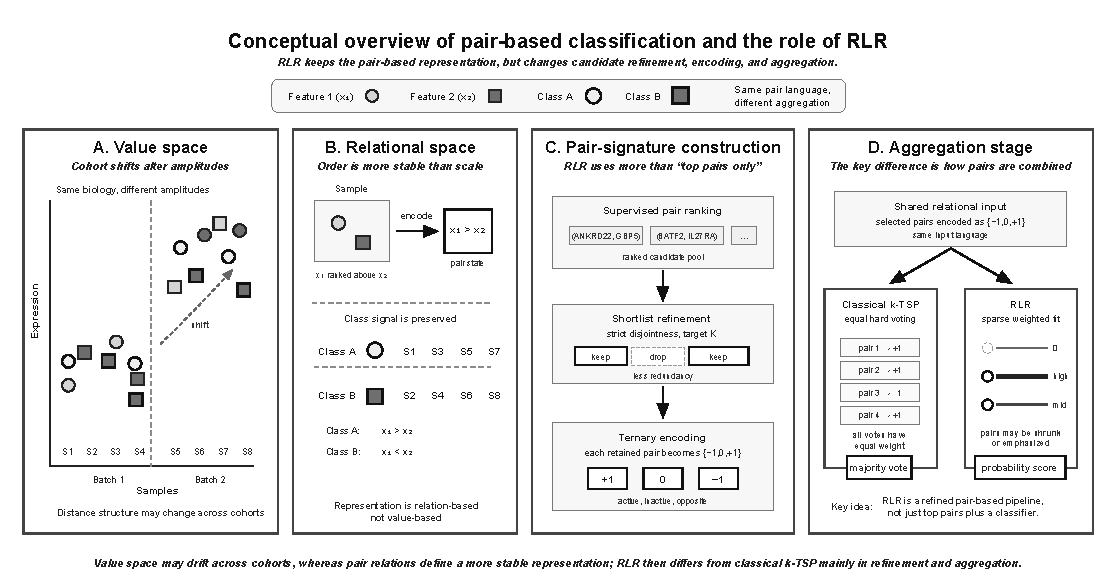
\includegraphics[width=\textwidth]{fig_methodolog3.pdf}
\caption{Conceptual overview of pair-based classification and the role of RLR. 
(A) Models based on absolute expression values can be affected by cohort-, platform-, or preprocessing-related changes in measurement scale. 
(B) Pair-based representations instead describe each sample through within-sample feature orderings, reducing dependence on absolute values while preserving relative information. 
(C) RLR constructs a relational feature space through supervised pair ranking, shortlist refinement with target size $K$, and margin-aware ternary encoding. 
(D) Classical $k$-TSP combines retained relations through equal hard voting, whereas RLR fits a sparse weighted probabilistic model over its shortlisted relational features. RLR should therefore be viewed as an integrated pair-based pipeline: it preserves an explicitly relational representation but differs from classical $k$-TSP in candidate refinement, encoding, and probabilistic fitting.}
\label{fig:conceptual_overview}
\end{figure*}

%%%%%%%%%%%%%%%%%%%%%%%%%%%%%%%%%%%%%%%%%
\section{Materials and Methods}\label{sec:methods}

\subsection{Study design, evaluation settings, and data sources}

The empirical study comprised four evaluation settings with deliberately different analytical roles: a multi-dataset benchmark for primary comparative inference, a fixed-split public-cohort case study for structural inspection, a leave-one-cohort-out cross-cohort stress test, and a classical benchmark for historical positioning.

\emph{CompCancer} served as the primary inferential benchmark and comprised 11 binary transcriptomic classification datasets. Each dataset was evaluated using stratified repeated 5-fold cross-validation. In the finalized benchmark protocol, nine datasets were evaluated with 10 repetitions, whereas West-2001 and Yeoh-2002-v1 were evaluated with 2 repetitions, yielding 470 outer test folds per model across the full benchmark. Performance was summarized within each dataset before formal cross-dataset statistical comparisons, so datasets rather than individual resampling folds constituted the inferential units. The dataset inventory and finalized repetition schedule are reported in the Supplementary Material.

The PTB data source comprised four publicly available Gene Expression Omnibus (GEO) cohorts: GSE19439, GSE19442, GSE19444, and GSE83456 \cite{Wu2025}. Following the cohort grouping used by Wu et al., GSE19439, GSE19442, and GSE19444 formed the discovery data (147 samples). The canonical \emph{PTB fixed-split setting} reported here uses the predefined discovery-data split of 103 training and 44 test samples from these three pooled cohorts. GSE83456 (106 samples) is the external validation cohort in the source benchmark, but it is not the test set used for the fixed-split results reported in this study; it is included in the separate leave-one-cohort-out analysis described below. The fixed-split setting was used primarily as a structural case study and was not treated as the main inferential basis of the study.

The \emph{PTB LOCO setting} used the same four GEO cohorts in a leave-one-cohort-out design. For each of the four runs, one complete cohort was held out for testing and the remaining three cohorts were used for model development. This setting was interpreted as a descriptive stress test under cohort-level distribution shift rather than as a source of formal comparative inference.

The auxiliary \emph{classical benchmark} comprised eight legacy binary microarray datasets: Adenocarcinoma, CNS, Colon, DLBCL, Leukemia, Ovarian, Breast2, and Prostate. These datasets were evaluated using repeated 5-fold cross-validation with 10 repetitions. The purpose of this benchmark was historical positioning under a protocol comparable to that used in earlier pair-based studies; results from this setting were therefore interpreted descriptively rather than as the primary evidence for RLR.

For both PTB settings, exhaustive pair scoring over the complete feature space was computationally impractical because of the substantially larger dimensionality. A median absolute deviation (MAD) prefilter was therefore applied within each training set to retain the 2000 most variable features before pair scoring. The feature ranking and selection were recomputed independently for every training split or cohort holdout, and no information from the corresponding test data was used during prefiltering.

Accordingly, \emph{CompCancer} provides the primary comparative and inferential evidence, the \emph{PTB fixed-split setting} supports structural inspection under a predefined discovery-data split, the \emph{PTB LOCO setting} evaluates descriptive cross-cohort robustness, and the classical benchmark provides historical context. The complete dataset inventory and protocol-specific details are provided in the Supplementary Material.

\subsection{Compared methods and model configurations}

The comparative analysis focused on a fixed set of pair-based classifiers chosen to examine the behavior of the proposed probabilistic relational pipeline relative to classical TSP-family baselines. The purpose of this comparison was not to identify the strongest classifier across all possible representation and model families, but to evaluate RLR within the methodological context from which it was developed.

As classical pair-based baselines, we included the Top-Scoring Pairs classifier (TSP$_1$) and three predefined configurations of the $k$-Top-Scoring Pairs ($k$-TSP) classifier: $k$-TSP-10, $k$-TSP-20, and $k$-TSP-50 \cite{Geman2004,Tan2005,Afsari2015}. These configurations represent compact, intermediate, and larger hard-voting pair signatures. The labels ``10'', ``20'', and ``50'' denote the configured number of retained pairwise rules used by the corresponding $k$-TSP models. In individual resampling splits, the realized number of retained pairs could be smaller when the requested configuration could not be fully constructed; structural summaries therefore distinguish nominal configuration size from the realized fitted structure where relevant.

RLR was evaluated in three corresponding main-text configurations: RLR-10, RLR-20, and RLR-50, with target shortlist sizes $K=10$, $K=20$, and $K=50$, respectively. All main-text RLR configurations used a rank-margin parameter of $m=10$, a strict gene-disjoint shortlist constraint ($d=2$), and an upstream candidate pool of the top 1000 ranked ordered relations. Under the strict disjointness setting, no gene can occur in more than one retained pair. Thus, the RLR labels indicate the target shortlist size $K$ and should not be interpreted as the number of relations that necessarily remain active after regularized fitting.

The resulting main comparison set consisted of TSP$_1$, $k$-TSP-10, $k$-TSP-20, $k$-TSP-50, RLR-10, RLR-20, and RLR-50. The $k$-TSP and RLR configurations with labels 10, 20, and 50 were compared at corresponding nominal pair-signature sizes, but the two model families differ not only in their final aggregation rule. RLR additionally uses margin-aware ternary encoding, a broader upstream candidate pool, gene-disjoint shortlist refinement, and regularized probabilistic fitting. Accordingly, the main comparisons should be interpreted as comparisons between the complete RLR pipeline and classical hard-voting pair-based baselines, rather than as an ablation isolating the effect of aggregation alone.

The main RLR configuration used $m=10$ throughout the primary analyses. Supplementary sensitivity analyses evaluate alternative rank-margin values and upstream candidate-pool sizes to characterize the robustness of this choice. In addition, an adaptive-$k$ hard-voting variant and post-hoc calibration of vote-derived $k$-TSP scores are reported as supplementary robustness and fairness checks. These analyses were not used to redefine the main comparison set.

For RLR, we distinguish four levels of model size: the upstream candidate-pool size, the target shortlist size $K$, the number of globally active relations after regularized fitting, and the number of locally active relations for an individual sample. These quantities describe different stages of the fitted model and are therefore reported separately in the structural analyses.

\subsection{Relative Logistic Regression}

Let $x=(x_1,\dots,x_p)$ denote the feature vector for a sample, where $x_i$ is the measured abundance of feature $i$ and $p$ is the number of available features. Rather than using the absolute feature values directly, RLR represents each sample through within-sample pairwise orderings.

For each sample, within-sample ranks were computed using average ranks for ties. Let $\pi_x(i)$ denote the resulting rank assigned to feature $i$ in sample $x$. For an oriented pair of features $(i,j)$, we define the signed rank gap as
\[
\Delta_{ij}(x)=\pi_x(j)-\pi_x(i).
\]
The sign of this quantity is interpreted relative to the pair orientation learned from the training data; reversing the orientation of a pair reverses the sign convention. Because the implementation uses ascending within-sample ranks, larger measured abundance corresponds to a larger rank. The exported \texttt{ordered\_pair} string is therefore treated only as an internal orientation label for the sign convention and is not read as a literal abundance inequality between its two genes.

Given a rank-margin parameter $m$, the pair is encoded as a ternary relational feature
\[
r_{ij}(x)\in\{-1,0,+1\},
\]
where
\[
r_{ij}(x)=
\begin{cases}
+1, & \text{if } \Delta_{ij}(x)\ge m,\\
-1, & \text{if } \Delta_{ij}(x)\le -m,\\
0, & \text{if } |\Delta_{ij}(x)|<m.
\end{cases}
\]
Thus, $r_{ij}(x)=+1$ and $r_{ij}(x)=-1$ denote sufficiently separated rank states in the two opposite oriented directions, whereas $r_{ij}(x)=0$ denotes an inactive relation whose absolute rank separation is below the specified margin. Pair orientation therefore determines the sign convention used for fitting and interpretation.

Candidate relations were scored exclusively on the training data using the signed pair score returned by the switchBox implementation (\texttt{SWAP.CalculateSignedScore}, with no additional filtering). Candidate pairs were ranked primarily by the absolute signed score. Orientation was then assigned using the training data to make the sign convention consistent with the class-dependent ordering difference; the positive class was the second level of the training factor. This orientation affects only the sign used to encode the relational feature and its fitted coefficient; it does not change the underlying unordered gene pair. In the main RLR analyses, the top 1000 ranked oriented relations formed the upstream candidate pool before shortlist refinement.

Shortlist refinement was then performed using the strict disjointness setting ($d=2$). Candidate pairs were traversed in descending order of their supervised pair score. A pair $(i,j)$ was accepted only if neither $i$ nor $j$ had previously appeared in a higher-ranked retained pair. Once a pair was accepted, both genes were marked as unavailable for subsequent pairs. The procedure continued until $K$ pairs had been retained or the candidate pool had been exhausted. This construction yields a gene-disjoint relational shortlist and limits repeated reuse of the same high-ranking genes.

For a retained set of relations
\[
\mathcal{P}=\{(i_1,j_1),\dots,(i_K,j_K)\},
\]
each sample is represented as
\[
r(x)=
\big(
r_{i_1j_1}(x),\dots,r_{i_Kj_K}(x)
\big).
\]

RLR fits a logistic model to this relational representation. For binary classification, the probability of the positive class is
\[
\Pr(y=1\mid x)
=
\sigma\!\left(
\beta_0+
\sum_{(i,j)\in\mathcal{P}}
\beta_{ij}r_{ij}(x)
\right),
\]
where
\[
\sigma(z)=\frac{1}{1+e^{-z}},
\]
$\beta_0$ is the intercept, and $\beta_{ij}$ denotes the fitted coefficient associated with relation $(i,j)$. Unlike equal hard voting, this formulation allows shortlisted relations to contribute with different magnitudes and directions.

The coefficients were estimated using elastic-net penalized logistic regression with the mixing parameter fixed at $\alpha=0.5$. The regularization strength $\lambda$ was selected within the training data using \texttt{cv.glmnet}, with binomial deviance as the optimization criterion and \texttt{lambda.min} used for the final fit. The internal cross-validation used up to five folds, reduced when necessary according to the size of the minority class, with a minimum of two folds. No separate optimization of $\alpha$ was performed in the main analysis.

Equivalently, the fitted coefficients solve the penalized objective
\begin{equation}
\label{eq:rlr_objective}
\begin{aligned}
\min_{\beta_0,\boldsymbol{\beta}} \quad
& -\frac{1}{N}\sum_{n=1}^{N}
\Big[
y_n \log \hat{p}_n
+(1-y_n)\log(1-\hat{p}_n)
\Big] \\
& \quad + \lambda
\left(
\alpha \lVert \boldsymbol{\beta} \rVert_1
+\frac{1-\alpha}{2}\lVert \boldsymbol{\beta} \rVert_2^2
\right),
\end{aligned}
\end{equation}
where $\hat{p}_n=\Pr(y_n=1\mid x^{(n)})$, $\lambda\ge0$ controls the overall regularization strength, and $\alpha\in[0,1]$ determines the balance between the $L_1$ and $L_2$ penalties.

All data-dependent operations, including feature prefiltering where applicable, pair scoring, candidate ranking, shortlist construction, internal selection of $\lambda$, and final coefficient estimation, were performed using only the training portion of the corresponding outer split or cohort holdout. The outer test data were used only for final evaluation.

The regularized fit can assign different importance to shortlisted relations and can shrink some coefficients exactly to zero. Consequently, the nominal shortlist size $K$ need not equal the number of relations contributing to the fitted model. RLR should therefore be interpreted as a sparse probabilistic model over a deliberately constructed pair-based relational feature space, rather than as logistic regression applied directly to the original omics measurements.


\subsection{Global relational structure and local active evidence}

For structural interpretation, we distinguish between four quantities that describe different stages of the RLR pipeline: the upstream candidate pool, the nominal target shortlist size $K$, the globally active fitted relations, and the subset of those relations that are active for a particular sample.

We define the \emph{global active structure} as the subset of shortlisted relations with non-zero fitted coefficients,
\[
\mathcal{P}_{\mathrm{active}}
=
\{(i,j)\in\mathcal{P}:\beta_{ij}\neq 0\}.
\]

For a sample $x$, we define the \emph{locally active relational set} as
\[
\mathcal{P}_{\mathrm{local}}(x)
=
\{(i,j)\in\mathcal{P}_{\mathrm{active}}:r_{ij}(x)\neq 0\}.
\]
Thus, a relation is locally active only if it is retained by the fitted model and its ternary encoding is non-zero for the sample under consideration.

Accordingly, a nominal configuration such as RLR-50 does not imply that 50 relations contribute to every fitted model or every individual prediction. Regularization may reduce the globally active structure below the target shortlist size, and the rank-margin encoding may further reduce the number of relations that are active for a specific sample.

These distinctions are used only to describe the effective relational structure of the fitted model and should not be interpreted as a separate local explanation algorithm. In the reported structural summaries, we therefore distinguish the number of globally active relations, the number of unique genes involved in those relations, and the distribution of locally active relations across samples, including the mean, median, and interquartile range.

\subsection{Evaluation metrics}

Predictive performance was evaluated using the area under the receiver operating characteristic curve (AUC), the F1-score, logarithmic loss (logloss), Brier score, and Expected Calibration Error (ECE). AUC was used to assess threshold-independent ranking performance \cite{Hanley1982}. For RLR, class labels used for F1 were obtained by thresholding the fitted positive-class probability at 0.5. For classical $k$-TSP, F1 was calculated from the class labels returned directly by \texttt{SWAP.KTSP.Classify}; it was not recomputed by thresholding the vote-derived score used for the probability-oriented metrics.

For classical $k$-TSP, the score used for AUC, logloss, Brier score, and ECE was derived from \texttt{SWAP.KTSP.Statistics}. If $k_{\mathrm{real}}$ denotes the realized number of retained pairs and $s(x)$ the returned voting statistic, the score was mapped to the unit interval as
\[
p(x)=\frac{s(x)+k_{\mathrm{real}}}{2k_{\mathrm{real}}}.
\]
Score orientation was determined using the training data only: when the mean derived score was lower in the positive training class than in the negative training class, the test score was replaced by $1-p(x)$. RLR instead produces a continuous positive-class probability directly from the fitted logistic model.

Logloss was treated as a central evaluation metric because one of the principal objectives of RLR is to provide a more flexible probabilistic integration of pair-based evidence. Before logloss calculation, scores were clipped to $[10^{-15},1-10^{-15}]$ to avoid numerical singularities. Models with similar discrimination or thresholded classification performance can nevertheless differ substantially in the scores assigned to individual predictions; logloss therefore complements AUC and F1 by using the full predictive score and strongly penalizing confident errors.

Probability-oriented performance was further assessed using the Brier score and Expected Calibration Error (ECE) \cite{VanCalster2019}. The Brier score was the mean squared difference between the predicted positive-class score and the observed binary outcome. ECE used 10 equal-width bins over $[0,1]$; empty bins were omitted, and each non-empty bin contributed its sample-frequency weight multiplied by the absolute difference between the mean predicted score and the empirical positive-class frequency in that bin. The same probability-metric definitions were applied to both model families.

For the auxiliary classical benchmark, accuracy was additionally reported to preserve comparability with the historical evaluation protocol used in earlier pair-based studies. Results in this benchmark are summarized as mean accuracy $\pm$ standard deviation across repeated cross-validation runs.

Beyond predictive performance, we characterized the fitted relational models using the number of globally active pairs, the number of unique genes represented in the active structure, the distribution of locally active relations across samples, and hub-concentration summaries where applicable.

\subsection{Statistical analysis}

Formal statistical comparisons were restricted to the \emph{CompCancer} benchmark, which served as the primary setting for comparative inference across multiple datasets. For each method and metric, resampling results were first aggregated within each dataset, yielding one summary value per dataset. Pairwise statistical comparisons were then performed across the 11 datasets, so that datasets rather than individual cross-validation folds constituted the inferential units. This avoided treating correlated repeated-resampling results from the same dataset as independent observations.

The paper-focus comparisons contrasted RLR-10 with $k$-TSP-10, RLR-20 with $k$-TSP-20, and RLR-50 with $k$-TSP-50. For each comparison and metric, paired differences across datasets were assessed using the Wilcoxon signed-rank test \cite{Wilcoxon1945} with datasets as the paired units. The analysis configuration additionally included the technical RLR-50 $d=2$ versus $d=1$ comparison. Holm adjustment \cite{Holm1979} was applied within the \emph{CompCancer} world to the complete configured family of 20 tests (four comparisons across five metrics); the three RLR-versus-$k$-TSP comparisons constitute the paper-focus subset. Raw and adjusted $p$-values are interpreted together with the corresponding dataset-level paired values and mean and median paired differences.

Interpretation emphasized the magnitude and consistency of dataset-level differences rather than statistical significance alone. Particular attention was given to logloss and the other probability-oriented metrics because these measures most directly reflect the intended probabilistic role of RLR, whereas AUC and F1 were used to assess whether changes in score quality were accompanied by changes in discrimination or thresholded classification performance.

The \emph{PTB fixed-split setting}, the \emph{PTB LOCO setting}, and the auxiliary classical benchmark were interpreted descriptively rather than inferentially. These settings were used to examine structural behavior, cross-cohort consistency, and historical positioning, respectively, and no formal hypothesis tests were used to support the primary conclusions from them. Detailed dataset-level comparisons, raw and Holm-adjusted $p$-values, and paired differences for \emph{CompCancer} are reported in the Supplementary Material.
%%%%%%%%%%%%%%%%%%%%%%%%%%%%%%%%%%%%%%%%%%%%%%%%%%%%%%%

\section{Results}\label{sec:results}

\subsection{Predictive performance across the three primary evaluation settings}

Table~\ref{tab:world_performance} and Fig.~\ref{fig:score_quality} summarize predictive performance across the three primary evaluation settings. Table~\ref{tab:world_performance} reports AUC, F1, and logloss, whereas Fig.~\ref{fig:score_quality} emphasizes the probability-oriented metrics. Across these settings, the most consistent differences in favor of RLR were observed for logloss, with generally similar tendencies for Brier score and expected calibration error. Differences in AUC and F1 were smaller and more setting-dependent.

\begin{figure*}[t]
\centering
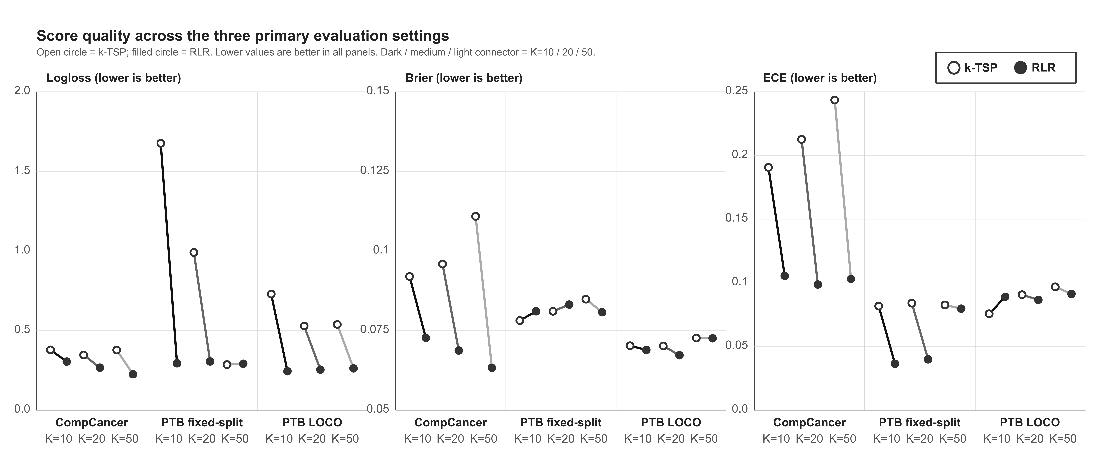
\includegraphics[width=\textwidth]{fig1score.pdf}
\caption{Probability-oriented performance across the three primary evaluation settings. RLR generally achieved lower logloss than the corresponding hard-voting $k$-TSP configurations, with broadly similar tendencies for Brier score and expected calibration error. The figure therefore emphasizes the probability-quality aspect of the comparison rather than suggesting uniform improvement across all predictive metrics.}
\label{fig:score_quality}
\end{figure*}

\begin{table*}[t]
\centering
\caption{Aggregate predictive performance across the three primary evaluation settings. RLR-10, RLR-20, and RLR-50 denote configurations with target shortlist sizes $K=10$, $K=20$, and $K=50$, respectively, using margin-aware ternary encoding ($m=10$), strict disjointness ($d=2$), and an upstream candidate pool of 1000 ranked relations. Classical $k$-TSP baselines are shown at the corresponding nominal pair-signature sizes. Brier score and expected calibration error are summarized in Fig.~\ref{fig:score_quality} and in the Supplementary Material.}
\label{tab:world_performance}
\small
\setlength{\tabcolsep}{4pt}
\begin{tabular}{lccc|ccc|ccc}
\toprule
& \multicolumn{3}{c|}{\textbf{CompCancer}}
& \multicolumn{3}{c|}{\textbf{PTB fixed-split}}
& \multicolumn{3}{c}{\textbf{PTB LOCO}} \\
\cmidrule(lr){2-4} \cmidrule(lr){5-7} \cmidrule(l){8-10}
\textbf{Method} & \textbf{AUC} & \textbf{F1} & \textbf{Logloss}
                & \textbf{AUC} & \textbf{F1} & \textbf{Logloss}
                & \textbf{AUC} & \textbf{F1} & \textbf{Logloss} \\
\midrule
$k$-TSP-10 & 0.956 & 0.860 & 0.378
           & 0.934 & 0.900 & 1.677
           & 0.959 & 0.899 & 0.730 \\

RLR-10     & 0.951 & 0.853 & 0.305
           & 0.930 & 0.900 & 0.294
           & \textbf{0.962} & 0.886 & \textbf{0.245} \\
\midrule
$k$-TSP-20 & 0.960 & 0.872 & 0.347
           & 0.935 & 0.900 & 0.991
           & 0.958 & 0.884 & 0.529 \\

RLR-20     & 0.955 & 0.867 & 0.267
           & 0.918 & 0.900 & 0.306
           & 0.957 & \textbf{0.909} & 0.254 \\
\midrule
$k$-TSP-50 & \textbf{0.963} & \textbf{0.884} & 0.378
           & \textbf{0.950} & 0.895 & \textbf{0.286}
           & 0.958 & 0.887 & 0.539 \\

RLR-50     & 0.957 & 0.869 & \textbf{0.226}
           & 0.944 & 0.895 & 0.292
           & 0.961 & 0.889 & 0.263 \\
\bottomrule
\end{tabular}
\end{table*}

In the repeated cross-validation \emph{CompCancer} benchmark, which provided the primary basis for comparative inference, RLR achieved lower aggregate logloss than the corresponding $k$-TSP configuration at all three target shortlist sizes. Logloss decreased from 0.378 to 0.305 for the 10-pair comparison, from 0.347 to 0.267 for the 20-pair comparison, and from 0.378 to 0.226 for the 50-pair comparison. Brier score and ECE showed broadly consistent probability-oriented patterns. By contrast, AUC and F1 were slightly higher for the corresponding hard-voting baselines in all three CompCancer comparisons. Thus, the main benchmark supports a specific advantage in score quality rather than uniform improvement in discrimination or thresholded classification performance.

Dataset-level analyses provided a more detailed view of this pattern. Paired comparisons across the 11 CompCancer datasets showed that differences were most consistent for logloss and related probability-oriented measures, whereas AUC and F1 effects were smaller and less uniform across datasets. Supplementary reliability analyses were consistent with this interpretation: lower Brier scores for RLR were associated primarily with a smaller reliability component in pooled out-of-fold summaries. An exploratory adaptive-$k$ hard-voting analysis likewise did not remove the main difference in probability-oriented performance, although the selected hard-voting signatures were often substantially smaller than their allowed upper limits. Detailed dataset-level comparisons and statistical summaries are reported in the Supplementary Material.

As a further fairness check, we evaluated post-hoc calibration of $k$-TSP vote-derived scores in the \emph{CompCancer} benchmark using calibration models fitted exclusively within the outer training data. Platt scaling substantially improved the probability-oriented performance of $k$-TSP. For the compact comparison, the resulting logloss was nearly identical to that of RLR-10 (0.308 vs.\ 0.305). For the 20- and 50-pair configurations, however, larger differences remained: Platt-calibrated $k$-TSP reached logloss values of 0.333 and 0.326, compared with 0.267 and 0.226 for RLR-20 and RLR-50, respectively. Isotonic calibration was less stable, particularly for logloss. These results indicate that part of the difference between classical vote-derived scores and RLR can be reduced by post-hoc calibration, but that calibration alone did not reproduce the probability-oriented performance of the larger RLR configurations.

In the \emph{PTB fixed-split setting}, the compact and intermediate RLR configurations again showed substantially lower logloss than the corresponding hard-voting models while preserving the same F1. RLR-10 reduced logloss from 1.677 to 0.294, and RLR-20 from 0.991 to 0.306. Their AUC values were slightly lower than those of the corresponding $k$-TSP models. At the larger configuration, the two approaches were broadly similar: $k$-TSP-50 and RLR-50 achieved logloss values of 0.286 and 0.292, respectively, with identical F1 and only a small AUC difference. Because this setting consists of a single predefined train/test split of the pooled discovery data rather than an independent external-validation test, these results are interpreted descriptively and primarily support the subsequent structural analyses. Pair-level comparisons, fitted coefficients, and local-activity summaries are reported in the Supplementary Material.

The \emph{PTB LOCO} analysis showed a similar probability-oriented tendency under cohort-level distribution shift. RLR achieved lower aggregate logloss at all three shortlist sizes: 0.245 versus 0.730 at $K=10$, 0.254 versus 0.529 at $K=20$, and 0.263 versus 0.539 at $K=50$. Differences in AUC were small, while F1 varied by configuration; RLR-20 achieved the highest F1 among the reported LOCO configurations. Because only four cohorts contributed to this analysis, the LOCO results are treated as descriptive evidence of cross-cohort behavior rather than as formal evidence of transportability.

Overall, the three evaluation settings support a deliberately narrow interpretation. The clearest empirical advantage of RLR concerns probability-oriented score quality, particularly logloss. Effects on AUC and F1 are smaller and depend on the dataset and configuration. RLR should therefore be interpreted as a probabilistic refinement of pair-based classification rather than as a uniformly superior classifier across all predictive criteria.

\subsection{Historical positioning under the classical benchmark protocol}

To provide historical context, we additionally evaluated RLR on the classical eight-dataset microarray benchmark and report the RLR-50 results alongside previously published values for established pair-based and conventional classifiers. This auxiliary analysis was not used as an inferential basis for the paper. Its purpose was to place RLR within a benchmark tradition commonly used in earlier TSP-family studies and to provide a qualitative indication of its historical performance range.

\begin{table*}[t]
\centering
\caption{Historical comparison on the auxiliary eight-dataset microarray benchmark. Results are reported as mean accuracy $\pm$ standard deviation (\%). Values for CDBP, $k$-TSP, M-$k$-TSP, Weight-$k$-TSP, VH-$k$-TSP, SVM-RFE, RS-SVM, RF, and $k$-NN are reproduced from Huang et al., whereas the RLR column reports results obtained in the present study for RLR-50 ($K=50$, $m=10$, $d=2$). Because the literature values and RLR results were not generated within a single unified experimental pipeline, the table is intended for historical context rather than controlled head-to-head comparison.}
\label{tab:legacy8_historical}
\resizebox{\textwidth}{!}{ \begin{tabular}{lcccccccccc} \toprule \textbf{Dataset} & \textbf{CDBP} & \textbf{$k$-TSP} & \textbf{M-$k$-TSP} & \textbf{Weight-$k$-TSP} & \textbf{VH-$k$-TSP} & \textbf{SVM-RFE} & \textbf{RS-SVM} & \textbf{RF} & \textbf{$k$-NN} & \textbf{RLR} \\ \midrule Adenocarcinoma & $82.66 \pm 3.77$ & $73.79 \pm 4.39$ & $78.47 \pm 3.38$ & $85.32 \pm 2.61$ & $82.50 \pm 2.63$ & $76.24 \pm 3.05$ & $77.98 \pm 4.82$ & $84.47 \pm 0.92$ & $82.95 \pm 0.92$ & $85.78 \pm 4.90$ \\ CNS & $57.17 \pm 5.24$ & $52.73 \pm 6.40$ & $52.57 \pm 6.16$ & $52.87 \pm 6.17$ & $58.13 \pm 4.92$ & $60.33 \pm 4.56$ & $62.10 \pm 5.07$ & $62.60 \pm 3.07$ & $56.77 \pm 5.26$ & $59.78 \pm 9.95$ \\ Colon & $95.97 \pm 1.50$ & $95.87 \pm 1.04$ & $95.55 \pm 1.24$ & $93.23 \pm 2.61$ & $95.42 \pm 1.40$ & $86.61 \pm 3.06$ & $89.43 \pm 3.71$ & $85.65 \pm 3.31$ & $81.26 \pm 3.24$ & $82.31 \pm 8.90$ \\ DLBCL & $94.68 \pm 1.71$ & $95.61 \pm 0.98$ & $95.19 \pm 1.09$ & $94.23 \pm 1.91$ & $95.74 \pm 1.58$ & $89.92 \pm 2.97$ & $94.18 \pm 2.13$ & $88.31 \pm 1.91$ & $85.06 \pm 2.91$ & $96.62 \pm 4.23$ \\ Leukemia & $96.25 \pm 1.64$ & $96.47 \pm 1.09$ & $96.14 \pm 1.35$ & $92.25 \pm 1.90$ & $95.31 \pm 1.25$ & $92.97 \pm 2.47$ & $97.52 \pm 1.14$ & $95.81 \pm 1.87$ & $91.97 \pm 1.89$ & $96.70 \pm 3.72$ \\ Ovarian & $87.96 \pm 3.11$ & $84.67 \pm 3.45$ & $85.11 \pm 2.72$ & $67.89 \pm 4.51$ & $86.22 \pm 2.93$ & $87.78 \pm 3.74$ & $94.21 \pm 2.37$ & $89.85 \pm 1.72$ & $85.78 \pm 2.79$ & $88.15 \pm 8.77$ \\ Breast2 & $61.35 \pm 4.38$ & $62.13 \pm 3.28$ & $62.16 \pm 3.20$ & $56.26 \pm 5.44$ & $60.99 \pm 3.30$ & $59.97 \pm 4.63$ & $66.16 \pm 3.70$ & $63.32 \pm 3.81$ & $60.62 \pm 3.01$ & $63.12 \pm 11.39$ \\ Prostate & $92.29 \pm 1.03$ & $92.18 \pm 1.16$ & $91.78 \pm 1.20$ & $86.57 \pm 2.95$ & $92.75 \pm 0.79$ & $91.78 \pm 2.36$ & $91.32 \pm 1.74$ & $89.53 \pm 1.80$ & $84.02 \pm 1.76$ & $91.22 \pm 5.65$ \\ \midrule Average & $83.54$ & $81.68$ & $82.12$ & $78.58$ & $83.38$ & $80.70$ & $84.11$ & $82.44$ & $78.55$ & $82.96$ \\ \bottomrule \end{tabular} }
\end{table*}

The historical results were heterogeneous. RLR-50 achieved an average accuracy of 82.96\% across the eight datasets, placing it within the overall range of the previously reported methods but not among the strongest approaches on average. Its relative performance also varied substantially by dataset. RLR-50 achieved numerically high accuracy on Adenocarcinoma and DLBCL and remained close to the strongest reported value on Leukemia, whereas its performance was substantially weaker on Colon and was not among the leading results on CNS, Ovarian, Breast2, or Prostate.

These results are therefore best interpreted as historical positioning rather than confirmatory evidence for the primary RLR claims. In particular, this benchmark does not reproduce the probability-oriented comparison investigated in \emph{CompCancer}, and differences between the literature values and the present RLR results should not be interpreted as formal evidence of superiority or inferiority. Instead, the benchmark shows that RLR can be situated within the performance range of classical pair-based omics classifiers while exhibiting considerable dataset-level heterogeneity.

A complete dataset-level summary of the auxiliary benchmark is provided in the Supplementary Material.

\subsection{Structural footprint, global active structure, and local activity}

\begin{table*}[t]
\centering
\caption{Aggregate structural summaries across the three primary evaluation settings. \emph{Global active pairs} denotes the number of shortlisted relations with non-zero fitted coefficients. \emph{Unique genes} reports the number of genes represented in the globally active relational structure. \emph{Local active mean} and \emph{local active median} summarize the number of globally active relations whose ternary encoding is non-zero for individual samples. Values are descriptive summaries and should be interpreted jointly with predictive performance rather than as independent measures of model quality.}
\label{tab:world_structure}
\small
\setlength{\tabcolsep}{6pt}
\begin{tabular}{llcccc}
\toprule
\textbf{Setting} & \textbf{Method} &
\textbf{Global active pairs} &
\textbf{Unique genes} &
\textbf{Local active mean} &
\textbf{Local active median} \\
\midrule
\multirow{6}{*}{CompCancer}
& $k$-TSP-10 & 10.00 & 20.00 & 10.00 & 10.00 \\
& RLR-10     & 9.31  & 18.62 & 8.41  & 8.63 \\
& $k$-TSP-20 & 20.00 & 40.00 & 20.00 & 20.00 \\
& RLR-20     & 16.63 & 33.26 & 15.10 & 15.34 \\
& $k$-TSP-50 & 49.27 & 98.55 & 49.27 & 49.27 \\
& RLR-50     & 28.09 & 56.19 & 25.55 & 25.92 \\
\midrule
\multirow{6}{*}{PTB fixed-split}
& $k$-TSP-10 & 10.00 & 20.00 & 10.00 & 10.00 \\
& RLR-10     & 8.00  & 16.00 & 7.93  & 8.00 \\
& $k$-TSP-20 & 20.00 & 40.00 & 20.00 & 20.00 \\
& RLR-20     & 13.00 & 26.00 & 12.77 & 13.00 \\
& $k$-TSP-50 & 50.00 & 100.00 & 50.00 & 50.00 \\
& RLR-50     & 21.00 & 42.00 & 20.52 & 21.00 \\
\midrule
\multirow{6}{*}{PTB LOCO}
& $k$-TSP-10 & 10.00 & 20.00 & 10.00 & 10.00 \\
& RLR-10     & 9.25  & 18.50 & 9.14  & 9.25 \\
& $k$-TSP-20 & 20.00 & 40.00 & 20.00 & 20.00 \\
& RLR-20     & 15.25 & 30.50 & 14.98 & 15.25 \\
& $k$-TSP-50 & 50.00 & 100.00 & 50.00 & 50.00 \\
& RLR-50     & 18.25 & 36.50 & 17.87 & 18.25 \\
\bottomrule
\end{tabular}
\end{table*}

Table~\ref{tab:world_structure} summarizes the effective relational structure across the three primary evaluation settings.

We next examined the effective relational structure of the fitted models. This analysis complements predictive performance by distinguishing the nominal configuration size from the number of relations retained after regularized fitting and from the subset of relations active for individual samples. These quantities are particularly relevant for RLR because the upstream candidate pool, target shortlist size, globally active fitted structure, and sample-level relational activity represent different stages of the modeling pipeline.

Across the three primary evaluation settings, regularized fitting reduced the effective RLR structure below its nominal target shortlist size, particularly for the larger configurations. In the \emph{CompCancer} benchmark, for example, the nominal RLR-50 configuration contained on average 28.1 globally active relations after fitting, compared with 49.3 retained relations for $k$-TSP-50. The corresponding mean number of locally active RLR relations was 25.5 per sample. The reduction was more pronounced in the PTB settings: RLR-50 retained 21 globally active relations in the fixed-split analysis and an average of 18.3 in the LOCO setting, compared with approximately 50 retained relations for the corresponding hard-voting models.

The distinction between nominal and effective model size is important for interpreting RLR. The upstream candidate pool and target shortlist determine the relational feature space available to the model, but elastic-net fitting may subsequently shrink shortlisted relations to zero. For an individual sample, ternary margin encoding may further render some globally retained relations inactive. Consequently, an RLR configuration labeled by $K$ should not be interpreted as using $K$ equally contributing relations in every prediction.

This structural sparsity does not imply that RLR is globally simpler than classical $k$-TSP. RLR includes additional candidate-ranking, shortlist-construction, and regularized-fitting stages, and its fitted coefficients introduce a richer aggregation mechanism than equal hard voting. The structural result is narrower: despite this additional modeling machinery, the final relational representation remains directly inspectable, and the number of relations active in the fitted model---and for an individual sample---can be substantially smaller than the nominal shortlist size.


\subsection{Structural inspection in the PTB fixed-split case study}

The \emph{PTB fixed-split setting} was used primarily for structural inspection rather than as a basis for broad predictive claims. We focus first on the compact $k$-TSP-10 and RLR-10 configurations because they provide readily inspectable pair-based signatures and illustrate how the effective relational structure changes under the RLR pipeline.

At the predictive level, the two models achieved the same F1-score (0.900), while RLR-10 yielded substantially lower logloss (0.294 vs.\ 1.677) and a slightly lower AUC (0.930 vs.\ 0.934). Thus, the compact PTB comparison follows the broader pattern observed in the primary analyses: the clearest difference concerns probability-oriented score quality rather than uniform improvement across predictive metrics.

The structural difference is also apparent. The $k$-TSP-10 model retained 10 disjoint pairwise rules that entered the hard-voting decision with equal weight. RLR-10 had a nominal target shortlist size of 10, but only 8 relations retained non-zero coefficients after regularized fitting. Sample-level activity was reduced only slightly further, with a mean of 7.9 locally active relations per sample (median 8; range 7--8). The compact RLR model therefore retained the pair-based representation while concentrating its fitted structure on a smaller set of unequally weighted relations.

This comparison is shown in Fig.~\ref{fig:ptb_case_study}. The figure emphasizes the distinction between a fixed equal-vote signature and the fitted coefficient structure obtained with RLR; detailed pair-level values are provided in the Supplementary Material.

\begin{figure*}[t]
\centering
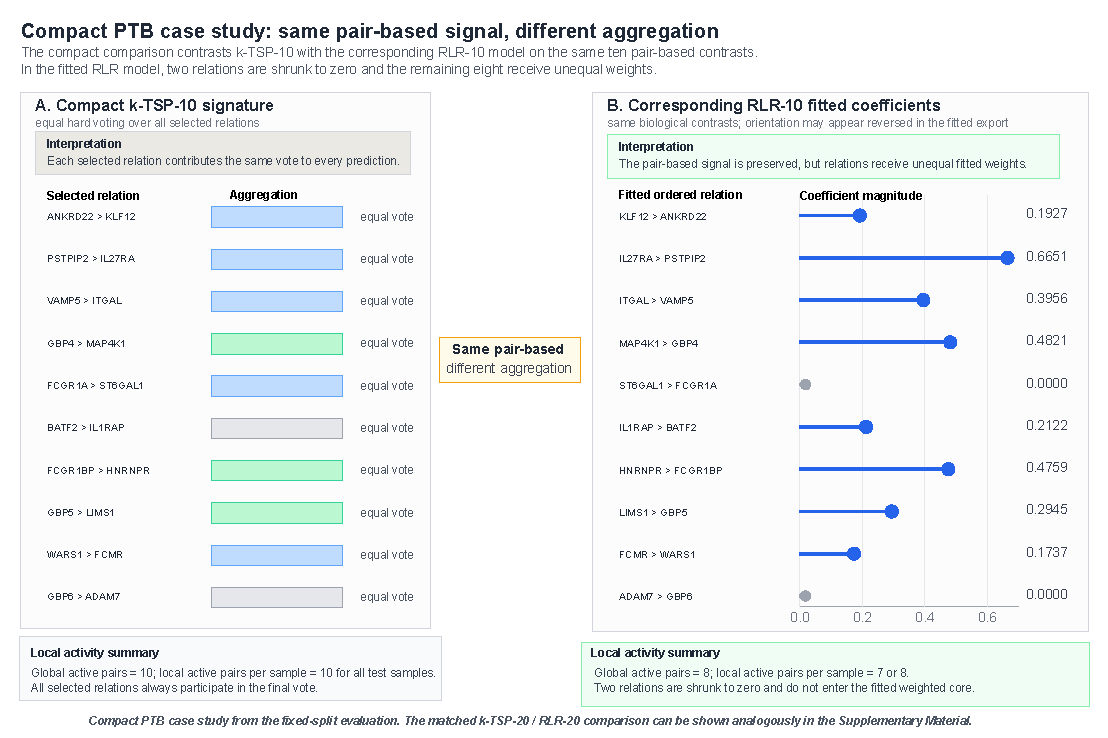
\includegraphics[width=\textwidth]{fig3_case.pdf}
\caption{Compact PTB fixed-split structural comparison. The left panel shows the ten selected relations in the $k$-TSP-10 signature, where retained pairs contribute equally to the hard-voting decision. The right panel shows the corresponding relational contrasts in the fitted RLR-10 model. Two relations receive zero coefficients, whereas the remaining eight receive unequal fitted weights. Ordered-pair orientation may appear reversed between model representations because relation direction determines the sign convention of the encoded feature. Pair strings shown in the exports are orientation labels and should not be interpreted as literal expression inequalities. The figure illustrates how RLR preserves an inspectable pair-based representation while producing a sparser weighted fitted structure.}
\label{fig:ptb_case_study}
\end{figure*}

The genes represented in the compact PTB signatures are broadly compatible with known host-response biology and include ANKRD22, PSTPIP2, IL27RA, BATF2, FCGR1-related signals, WARS1, and several GBP-family members. This observation is interpreted descriptively. The PTB analysis was designed to inspect the structure of the fitted relational models, not to identify or validate a diagnostic biomarker panel.

As an exploratory functional check, we performed over-representation analysis (ORA) using the training-only MAD-prefiltered PTB feature universe as the background set. In the intermediate $K=20$ comparison, all 40 $k$-TSP shortlist genes and all 26 RLR active genes were present in the 2000-gene background universe. The $k$-TSP-20 list yielded 20 FDR-significant terms across GO Biological Process, Hallmark, and Reactome, whereas the smaller RLR-20 active set yielded three significant Hallmark terms: allograft rejection, interferon-gamma response, and interferon-alpha response. Thus, both gene sets remained compatible with an immune/host-response interpretation, while the RLR active set produced fewer significant enrichment results. Because the analyzed gene sets differ substantially in size, the number of significant terms should not be interpreted as evidence of greater biological specificity or superiority of either model.

This exploratory comparison is summarized in Fig.~\ref{fig:ptb_ora}, with complete enrichment results and gene-set details provided in the Supplementary Material.

\begin{figure*}[t]
\centering
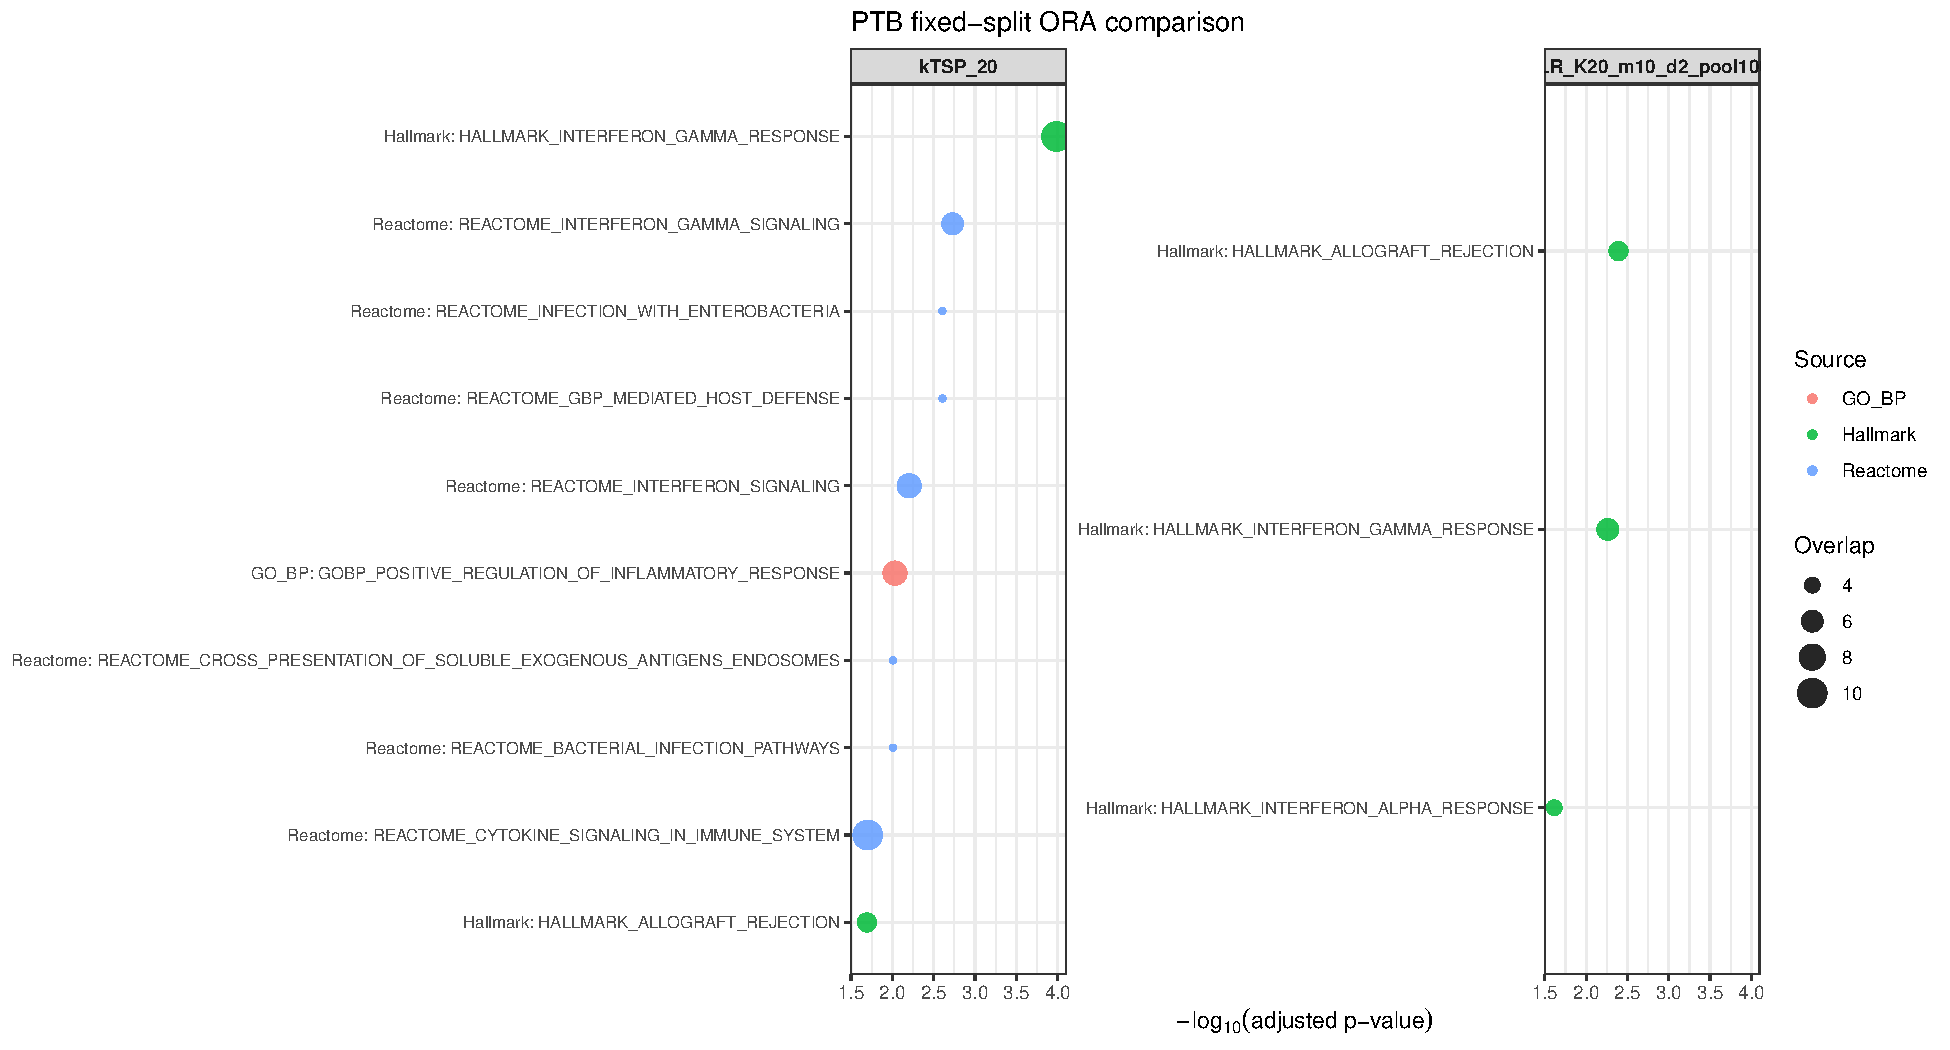
\includegraphics[width=\textwidth]{fig_ptb_fixed_ora_k20.pdf}
\caption{Exploratory functional-enrichment comparison for the intermediate PTB fixed-split signatures. ORA used the 2000-gene training-only MAD-prefiltered PTB universe as background. The $k$-TSP-20 shortlist yielded 20 FDR-significant terms across GO Biological Process, Hallmark, and Reactome, whereas the smaller RLR-20 active set yielded three significant Hallmark terms, including interferon-gamma and interferon-alpha responses. Point size indicates overlap size and the horizontal axis shows $-\log_{10}(\mathrm{adjusted}\ p\mathrm{-value})$. Because the analyzed gene sets differ in size, the figure is intended as descriptive functional support rather than as evidence of greater biological specificity of either model.}
\label{fig:ptb_ora}
\end{figure*}

A similar reduction in effective fitted structure was observed for the intermediate configuration. RLR-20 retained 13 relations with non-zero coefficients from a nominal target shortlist of 20, compared with 20 retained rules for $k$-TSP-20. Together with the compact comparison, this indicates that the distinction between nominal shortlist size and fitted active structure is not confined to a single RLR configuration.

\subsection{Summary of the empirical picture}

Taken together, the results support a specific and deliberately limited interpretation of RLR. In the primary \emph{CompCancer} benchmark, the clearest and most consistent differences relative to the corresponding hard-voting $k$-TSP configurations were observed in probability-oriented metrics, particularly logloss, whereas differences in AUC and F1 were smaller and more dataset-dependent. In the PTB analyses, RLR retained an inspectable pair-based representation while regularized fitting reduced the globally active structure below the nominal shortlist size and ternary encoding further limited the set of relations active for individual samples. In the auxiliary historical benchmark, RLR fell within the performance range of established pair-based methods but did not emerge as a uniformly leading approach.

Overall, the empirical evidence supports viewing RLR as an integrated probabilistic refinement of pair-based omics classification. Its principal demonstrated advantage lies in the quality of the resulting predictive scores and in the distinction between nominal, globally active, and locally active relational structure, rather than in universal superiority across all predictive criteria. Additional robustness, calibration, structural, functional, and historical analyses are reported in the Supplementary Material.



%%%%%%%%%%%%%%%%%%%%%%%%%%%%%%%
\section{Discussion}\label{sec:discussion}

The present study evaluated Relative Logistic Regression (RLR) as an integrated probabilistic extension of pair-based omics classification. RLR retains an explicitly relational representation based on within-sample feature comparisons, but combines supervised pair ranking, margin-aware ternary encoding, gene-disjoint shortlist construction, and sparse elastic-net logistic fitting within a single modeling pipeline. The empirical results do not support universal superiority across predictive criteria. Instead, the clearest and most consistent differences relative to the corresponding classical $k$-TSP configurations were observed in probability-oriented metrics, particularly logloss, whereas AUC and F1 were smaller in magnitude and more dependent on dataset and configuration.

\subsection{RLR as a probabilistic extension of pair-based modeling}

The motivation for RLR is not to replace pair-based classification with a conventional value-based learner, but to retain the relational representation while allowing the selected pairwise signals to contribute unequally within a regularized probabilistic model. Classical TSP-family methods derive much of their appeal from simple within-sample comparisons and compact decision rules. RLR preserves this representation but separates the nominal shortlist from the final fitted structure: shortlisted relations may receive different coefficients, may be shrunk to zero, and may be inactive for particular samples under the rank-margin encoding.

This distinction is important when interpreting the contribution of the method. The present experiments compare the complete RLR pipeline with classical hard-voting pair-based baselines; they do not isolate the causal contribution of each individual component. The results therefore support RLR as an integrated probabilistic refinement rather than demonstrating that the aggregation step alone is responsible for the entire observed performance difference.

\subsection{Why the clearest differences concern score quality}

The most consistent empirical advantage of RLR was observed in logloss, with broadly similar tendencies for Brier score and expected calibration error. This pattern is compatible with the different ways in which the compared model families generate prediction scores. Classical $k$-TSP produces discrete vote-derived scores, whereas RLR produces continuous probabilities from a jointly fitted regularized model. Models can therefore exhibit similar AUC or F1 while differing substantially in the scores assigned to individual predictions.

The primary \emph{CompCancer} benchmark showed this distinction most clearly. RLR achieved lower aggregate logloss at all three nominal shortlist sizes, whereas the corresponding $k$-TSP models retained slightly higher AUC and F1. The PTB analyses showed a similar probability-oriented tendency, although the larger fixed-split configuration was essentially neutral. These results argue against a generic ``better classifier'' interpretation and instead support a narrower conclusion centered on score quality.

The supplementary calibration analysis further qualifies this result. Platt scaling substantially improved the probability-oriented performance of classical $k$-TSP vote-derived scores and almost eliminated the compact $K=10$ logloss difference. Larger differences remained for the $K=20$ and $K=50$ configurations. Thus, part of the observed advantage is attributable to the coarse probability representation of uncalibrated vote-derived scores, while the remaining differences indicate that simple post-hoc remapping does not reproduce the behavior of the larger RLR models. Because RLR also differs from classical $k$-TSP in encoding, shortlist construction, and regularized fitting, these analyses should not be interpreted as identifying a single causal mechanism.

Probability-oriented performance may be relevant in applications in which model outputs are interpreted beyond a binary class label. However, the present study did not evaluate clinical decision utility, decision thresholds, net benefit, or prospective use. Improvements in logloss, Brier score, or ECE should therefore be interpreted as improvements in statistical score quality rather than direct evidence of improved clinical usefulness.

\subsection{Interpretability through fitted relational structure}

A second contribution of the study concerns the distinction between nominal and effective relational model size. In classical hard-voting models, retained relations directly define the voting rule. In RLR, the upstream candidate pool, target shortlist size, globally active fitted structure, and locally active relational set are distinct quantities.

The structural summaries illustrate this distinction particularly clearly for the larger RLR configurations. In \emph{CompCancer}, RLR-50 retained approximately 28 globally active relations on average from a nominal target shortlist of 50, with approximately 26 relations active per sample. In the PTB fixed-split analysis, the corresponding fitted structure contained 21 globally active relations, while the LOCO analysis yielded an average of approximately 18. These reductions arise first from regularized coefficient shrinkage and then, at the sample level, from the ternary margin encoding.

This should not be interpreted as showing that RLR is globally simpler than classical $k$-TSP. RLR introduces additional modeling stages and a richer fitted decision function. The narrower interpretability claim is that the final model remains directly inspectable at the level of gene-pair relations and coefficients, while the number of relations participating in the fitted model or a particular sample prediction may be substantially smaller than the nominal shortlist size.

The use of strict gene disjointness in the main RLR configurations further constrains repeated reuse of the same genes across retained pairs and makes the relationship between retained relations and participating genes straightforward. The present study does not establish that this constraint is universally optimal; rather, it forms part of the finalized RLR configuration evaluated here.

\subsection{Interpretation of the PTB case study}

The PTB fixed-split setting was used primarily for structural inspection. The compact comparison between $k$-TSP-10 and RLR-10 illustrates how the same general pair-based representation can lead to a different fitted decision structure. RLR-10 retained eight non-zero relations from a nominal target shortlist of ten and assigned unequal coefficients to the retained relations, while the corresponding hard-voting model used ten equally weighted rules.

The genes represented in these compact signatures are broadly compatible with host-response biology, including ANKRD22-, GBP-, FCGR1-, BATF2-, IL27RA-, and WARS1-related signals. The exploratory enrichment analysis likewise showed interferon- and host-response-related terms for both $k$-TSP and RLR-derived gene sets. Because the analyzed gene sets are small and differ in size, the smaller number of significant enrichment terms observed for RLR should not be interpreted as evidence of greater biological specificity or mechanistic validity. Its main value is to show that the reduced RLR active set remains compatible with the same broad biological theme as the original pair-based signature.

Accordingly, the PTB analysis provides an interpretable biomedical example of the fitted relational structure, but it should not be read as a biomarker-discovery study or as independent clinical validation of the identified gene pairs.

\subsection{How to interpret the complementary benchmarks}

The four evaluation settings serve deliberately different purposes. \emph{CompCancer} provides the primary basis for comparative inference across datasets. The \emph{PTB fixed-split} setting supports structural inspection under a predefined discovery-data train/test split, whereas the \emph{PTB LOCO} analysis provides descriptive evidence under stronger cohort-level distribution shift. With only four cohorts, the LOCO results should not be interpreted as definitive evidence of transportability.

The auxiliary eight-dataset benchmark serves a different purpose again. It places RLR within a historically familiar microarray benchmark landscape but combines newly generated RLR results with literature-reported values obtained outside a unified experimental pipeline. It therefore provides context rather than controlled comparative evidence. RLR-50 fell within the historical performance range of the reported methods but was not among the strongest methods overall. This reinforces the decision to anchor the main claims of the paper in the primary benchmark and structural analyses rather than in the auxiliary historical comparison.

\subsection{Limitations and future directions}

Several limitations should be considered when interpreting the results. First, the main comparison contrasts the complete RLR pipeline with classical $k$-TSP configurations. Because RLR differs in relational encoding, candidate-pool construction, shortlist refinement, and regularized fitting, the present design does not isolate the individual contribution of each component. A controlled component-wise ablation would be required to determine how much of the observed score-quality difference is attributable specifically to probabilistic aggregation.

Second, the primary benchmark is based on established transcriptomic datasets and repeated resampling rather than on a large contemporary multi-center external-validation study. The PTB fixed-split case study uses a predefined 103/44 train/test split of the pooled discovery cohorts and therefore does not constitute independent external validation. The LOCO analysis contains only four cohorts and likewise offers descriptive rather than definitive evidence of cross-study transportability.

Third, the comparison was intentionally centered on the pair-based methodological family. The study therefore does not establish superiority over broader value-based, deep-learning, or other unrelated omics classifiers, nor was it designed as a comprehensive benchmark across representation families.

Fourth, probability-oriented improvements should not be equated with demonstrated clinical utility. The study does not include prospective evaluation, clinical decision analysis, net-benefit assessment, or externally validated operating thresholds.

Fifth, the fitted relational structures are inspectable, but the biological analyses remain exploratory. The study was not designed to establish mechanistic relationships or validate diagnostic biomarkers, and the PTB enrichment results should therefore be interpreted conservatively.

Finally, the empirical evaluation is centered mainly on established bulk transcriptomic benchmarks. Future studies should examine whether the same modeling principles remain useful in larger multi-cohort datasets and in newer RNA-seq, multi-omics, or other high-dimensional biomedical settings.

Future methodological work could also examine alternative shortlist-construction strategies, relational encodings, and regularization schemes, as well as controlled ablations that separate their respective contributions. Further evaluation across heterogeneous external cohorts would help determine under which conditions probabilistic relational modeling provides the greatest advantage over classical pair-based voting.

Supplementary runtime analyses indicate that pair ranking constitutes the dominant computational cost of the current RLR pipeline, whereas shortlist refinement, relational encoding, and penalized fitting are comparatively inexpensive once the ranked candidate pool has been obtained.

\section{Conclusion}\label{sec:conclusion}

Relative Logistic Regression provides an integrated probabilistic extension of pair-based omics classification by combining relational feature construction with sparse regularized logistic fitting. Across the primary evaluation settings, its clearest and most consistent advantage over the corresponding classical $k$-TSP configurations was observed in probability-oriented score quality, particularly logloss, whereas differences in AUC and F1 were smaller and more setting-dependent.

The fitted RLR models also distinguish nominal shortlist size from globally and locally active relational structure, allowing the final pair-based representation to remain directly inspectable despite the richer probabilistic fitting procedure. The results therefore support RLR as a practical refinement of pair-based modeling rather than as a universally superior classifier. Further work should determine how the individual components of the pipeline contribute to performance and evaluate the approach across larger and more heterogeneous external cohorts.

\section*{Data and Code Availability}

All datasets analyzed in this study originate from publicly available sources described in the manuscript and Supplementary Material. The cleaned publication repository containing the RLR implementation, frozen experiment configurations, analysis scripts, reproducibility documentation, checksums, and selected reference outputs is available at \url{https://github.com/mczajkowskipb/relative-logistic-regression}. Data-acquisition and preprocessing instructions, including the documented provenance boundary for the historical legacy8 inputs, are provided in the repository.
\begin{thebibliography}{99}

\bibitem{Cox1958}
D.~R. Cox.
\newblock The regression analysis of binary sequences.
\newblock \emph{Journal of the Royal Statistical Society: Series B (Methodological)}, 20(2):215--232, 1958.

\bibitem{Wilcoxon1945}
F.~Wilcoxon.
\newblock Individual comparisons by ranking methods.
\newblock \emph{Biometrics Bulletin}, 1(6):80--83, 1945.

\bibitem{Holm1979}
S.~Holm.
\newblock A simple sequentially rejective multiple test procedure.
\newblock \emph{Scandinavian Journal of Statistics}, 6(2):65--70, 1979.

\bibitem{Hanley1982}
J.~A. Hanley and B.~J. McNeil.
\newblock The meaning and use of the area under a receiver operating characteristic (ROC) curve.
\newblock \emph{Radiology}, 143(1):29--36, 1982.

\bibitem{Tibshirani1996}
R.~Tibshirani.
\newblock Regression shrinkage and selection via the lasso.
\newblock \emph{Journal of the Royal Statistical Society: Series B (Methodological)}, 58(1):267--288, 1996.

\bibitem{ZouHastie2005}
H.~Zou and T.~Hastie.
\newblock Regularization and variable selection via the elastic net.
\newblock \emph{Journal of the Royal Statistical Society: Series B (Statistical Methodology)}, 67(2):301--320, 2005.

\bibitem{Friedman2010}
J.~Friedman, T.~Hastie, and R.~Tibshirani.
\newblock Regularization paths for generalized linear models via coordinate descent.
\newblock \emph{Journal of Statistical Software}, 33(1):1--22, 2010.

\bibitem{VanCalster2019}
B.~van Calster, D.~J. McLernon, M.~van Smeden, L.~Wynants, and E.~W. Steyerberg.
\newblock Calibration: the Achilles heel of predictive analytics.
\newblock \emph{BMC Medicine}, 17:230, 2019.

\bibitem{Gordon2002}
G.~J. Gordon, R.~V. Jensen, L.-L. Hsiao, S.~R. Gullans, J.~Blumenstock, R.~M. Ramaswamy, W.~G. Richards, D.~J. Sugarbaker, and R.~Bueno.
\newblock Translation of microarray data into clinically relevant cancer diagnostic tests using gene expression ratios in lung cancer and mesothelioma.
\newblock \emph{Cancer Research}, 62(17):4963--4967, 2002.

\bibitem{Bo2002}
T.-H. B{\o} and I.~Jonassen.
\newblock New feature subset selection procedures for classification of expression profiles.
\newblock \emph{Genome Biology}, 3(4):research0017, 2002.

\bibitem{Geman2004}
D.~Geman, C.~d'Avignon, D.~Q. Naiman, and R.~L. Winslow.
\newblock Classifying gene expression profiles from pairwise mRNA comparisons.
\newblock \emph{Statistical Applications in Genetics and Molecular Biology}, 3(1):Article 19, 2004.

\bibitem{Tan2005}
A.~C. Tan, D.~Q. Naiman, L.~Xu, R.~L. Winslow, and D.~Geman.
\newblock Simple decision rules for classifying human cancers from gene expression profiles.
\newblock \emph{Bioinformatics}, 21(20):3896--3904, 2005.

\bibitem{Lin2009}
X.~Lin, B.~Afsari, L.~Marchionni, L.~Cope, G.~Parmigiani, D.~Naiman, and D.~Geman.
\newblock The ordering of expression among a few genes can provide simple cancer biomarkers and signal BRCA1 mutations.
\newblock \emph{BMC Bioinformatics}, 10:256, 2009.

\bibitem{Eddy2010}
J.~A. Eddy, L.~Hood, N.~D. Price, and D.~Geman.
\newblock Identifying tightly regulated and variably expressed networks by Differential Rank Conservation (DIRAC).
\newblock \emph{PLoS Computational Biology}, 6(5):e1000792, 2010.

\bibitem{Magis2012}
A.~T. Magis and N.~D. Price.
\newblock The top-scoring `N' algorithm: a generalized relative expression classification method from small numbers of biomolecules.
\newblock \emph{BMC Bioinformatics}, 13:227, 2012.

\bibitem{Marchionni2013}
L.~Marchionni, B.~Afsari, D.~Geman, and J.~T. Leek.
\newblock A simple and reproducible breast cancer prognostic test.
\newblock \emph{BMC Genomics}, 14:336, 2013.

\bibitem{Afsari2015}
B.~Afsari, E.~J. Fertig, D.~Geman, and L.~Marchionni.
\newblock switchBox: an R package for k-Top Scoring Pairs classifier development.
\newblock \emph{Bioinformatics}, 31(2):273--274, 2015.

\bibitem{Kim2016}
S.~Kim, C.-W. Lin, and G.~C. Tseng.
\newblock MetaKTSP: a meta-analytic top scoring pair method for robust cross-study validation of omics prediction analysis.
\newblock \emph{Bioinformatics}, 32(13):1966--1973, 2016.

\bibitem{Moody2020}
L.~Moody, H.~Chen, and Y.-X. Pan.
\newblock Considerations for feature selection using gene pairs and applications in large-scale dataset integration.
\newblock \emph{BMC Medical Genomics}, 13(Suppl 10):148, 2020.

\bibitem{Kwan2023}
B.~Kwan, M.~Fu, A.~Higginbotham, S.~Potok, M.~M. Hannan, M.~Wolf, T.~M. Coffman, L.~P. RoyChoudhury, and M.~A. Cohen-Rosenblum.
\newblock A generalized covariate-adjusted top-scoring pair algorithm with applications to diabetic kidney disease stage classification in the Chronic Renal Insufficiency Cohort (CRIC) Study.
\newblock \emph{BMC Bioinformatics}, 24(1):57, 2023.

\bibitem{Cheng2023}
L.~Cheng, Y.~Liu, X.~Qian, Y.~Ma, M.~Zhang, X.~Xu, H.~Chen, X.~Zhang, J.~Zhu, H.~Li, Y.~Wang, and J.~Wang.
\newblock GPGPS: a robust prognostic gene pair signature of glioma ensembling IDH mutation and 1p/19q co-deletion.
\newblock \emph{Bioinformatics}, 39(1):btac850, 2023.

\bibitem{Chen2023}
Y.~Chen, H.~Zhang, and X.~Sun.
\newblock Improving the performance of single-cell RNA-seq data mining based on relative expression orderings.
\newblock \emph{Briefings in Bioinformatics}, 24(1):bbac556, 2023.

\bibitem{Yan2024}
J.~Yan, Q.~Zeng, and X.~Wang.
\newblock RankCompV3: a differential expression analysis algorithm based on relative expression orderings.
\newblock \emph{BMC Bioinformatics}, 25:259, 2024.

\bibitem{Xie2024iScience}
J.~Xie, Y.~Liu, Z.~Wang, Z.~Lin, X.~Sun, Y.~Xie, Z.~Qi, Y.~Zhu, M.~Zhang, X.~Yuan, J.~Jiang, and C.~Jin.
\newblock Deep learning model to discriminate diverse infection types based on pairwise analysis of host gene expression.
\newblock \emph{iScience}, 27(6):109908, 2024.

\bibitem{Wu2025}
C.~Wu, X.~Xie, X.~Yang, M.~Du, H.~Lin, and J.~Huang.
\newblock Applications of gene pair methods in clinical research: advancing precision medicine.
\newblock \emph{Molecular Biomedicine}, 6(1):22, 2025.

\bibitem{Zheng2025}
X.~Zheng, X.~Zhang, J.~Wang, Y.~Lin, X.~Sun, and Y.~Chen.
\newblock Less is more: relative rank is more informative than absolute abundance for compositional NGS data.
\newblock \emph{Briefings in Functional Genomics}, 24:elae045, 2025.

\bibitem{Jin2025}
N.~Jin, Y.~He, X.~Sun, J.~Xie, Y.~Zhu, C.~Wu, and J.~Huang.
\newblock PAGE-based transfer learning from single-cell to bulk sequencing enhances model generalization for sepsis diagnosis.
\newblock \emph{Briefings in Bioinformatics}, 26(1):bbae661, 2025.

\bibitem{Czajkowski2025}
M.~Czajkowski, K.~Jurczuk, and M.~Kretowski.
\newblock Enhancing transparency of omics data analysis with the evolutionary multi-test tree and relative expression.
\newblock \emph{Expert Systems with Applications}, 276:127131, 2025.

\bibitem{Aitchison1986}
J.~Aitchison.
\newblock \emph{The Statistical Analysis of Compositional Data}.
\newblock Chapman and Hall, London, 1986.

\bibitem{Wang2015}
H.~Wang, Q.~Sun, W.~Zhao, L.~Qi, Y.~Gu, P.~Li, M.~Zhang, Y.~Li, S.-L. Liu, and Z.~Guo.
\newblock Individual-level analysis of differential expression of genes and pathways for personalized medicine.
\newblock \emph{Bioinformatics}, 31(1):62--68, 2015.

\bibitem{Huang2022}
X.~Huang, Z.~Liao, B.~Liu, F.~Tao, B.~Su, and X.~Lin.
\newblock A novel method for constructing classification models by combining different biomarker patterns.
\newblock \emph{IEEE/ACM Trans. Comput. Biol. Bioinform.}, 19(2):786--794, Mar./Apr. 2022.
\newblock doi: 10.1109/TCBB.2020.3022076.
\end{thebibliography}


\end{document}